\begin{frame}{Lieb-Schultz-Mattis Theorem}
\vskip-1.5cm
 Featured states are 
 \bi 
 \item either gapless
 \item or spontaneously break spin symmetry
 \item or spontaneously break translational symmetry
 \item or topologically ordered
 \note{Why do we group these together? Shouldn't define a featureless insulator by what it is not.}
 \item {but always have (nearly) degenerate states when placed in periodic boundary conditions.}
 \ei 
 \note{This is a meaningful distinction because of the LSM}
 States with fractional charge per unit cell cannot be featureless.
\only<1>{
\begin{LSM}
A spin $1/2$ chain with $SU(2)$ and translational symmetry has a ground state that is either gapless or breaks symmetry.
\end{LSM}
}
\only<2>{
\begin{Oshikawa}
A particle-number conserving system with a fractional number of particles per unit cell cannot have a fixed energy gap on a torus.
The same holds for a $U(1)$-symmetric spin system with total spin $j$ per unit cell and magnetization $m$ per unit cell, with $j-m$ not integer. 
\end{Oshikawa}
}
\note{The argument for this is called the }
\only<3>{
\begin{block}{Proof:}
\begin{columns}[T]
\begin{column}[T]{0.6\textwidth}
{\em
The Lieb-Schultz-Mattis-Laughlin-Bonesteel-Affleck-Yamanaka-Oshikawa flux-threading argument}
\end{column}
\begin{column}[T]{0.4\textwidth}
\vskip-1.8cm
\begin{figure}
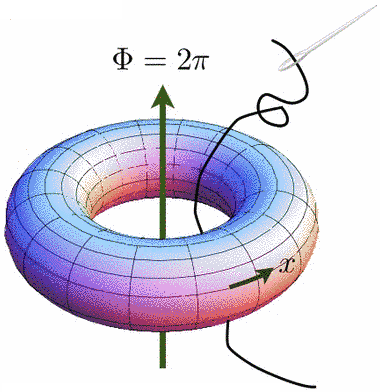
\includegraphics[width=0.9\columnwidth]{diagrams/flux-threading.png}
\end{figure}
\end{column}
\end{columns}
\end{block}
}
\end{frame}